\chapter{Data}
%présentation des datas, à quoi ça ressemble, preprocessing, data auxiliaire
Realizing that we need to be careful with time zones, as for example, TSLA is traded on the NASDAQ stock exchange, which is in New York, whereas Elon Musk tweets from California and I am in Switzerland while analysing the data and the reader might be anywhere in the world, we shall convert all times to UTC.
\section{Main data: Tesla Stock Price}
The \acrshort{tsla} price data was retrieved using the python package "yfiance" which makes calls to the Yahoo Finance \Gls{API}. We were able to download 730 days worth of hourly data, spanning the last 730 days from download date. The Yahoo Finance \Gls{API} is not being maintained, so this may not be possible in the future. The data was retrieved on February 10th 2021 and spanned from February 11th 2019 at 00:00 till February 10th 2021 at 00:00.
The raw data contained the following variables: "Open", "High", "Low", "Close", "Volume", "Dividends" and "Stock Splits".
For the purposes of this thesis, we only kept "Open" which was an arbitrary choice.

\begin{figure}[h]
	\centering
	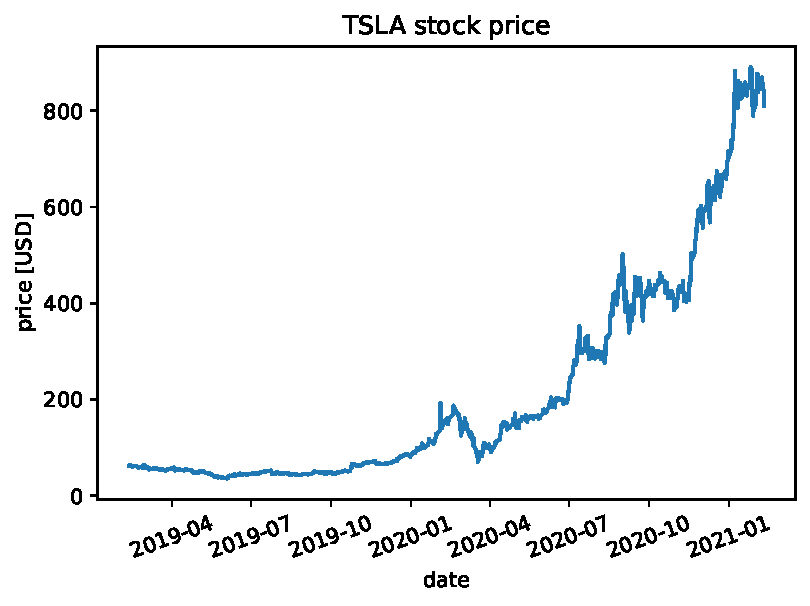
\includegraphics[width=\textwidth]{img/img_tsla.pdf}
	\caption{TSLA hourly opening stock price}
	\label{fig:tsla_open}
\end{figure}



\section{Auxiliary data}
\subsection{Google Trends}
\acrfull{gt} is a tool that lets researchers explore how the Google search engine as been used. We shall use the search term "tesla" in the explanation and graphics, as the other search terms ('tsla', 'tesla stock' and 'musk') were similarly preprocessed.

\begin{figure}[h]
	\centering
	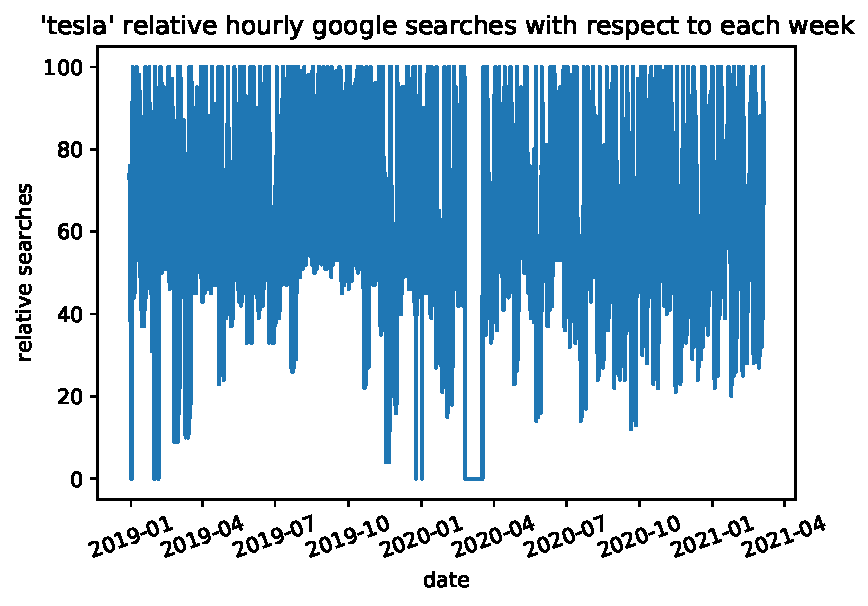
\includegraphics[width=\textwidth]{img/img_GT_tesla_raw.pdf}
	\caption{Hourly google searches of the term "tesla" relatively to each week, in percentage of the weekly maximum}
	\label{fig:GT_tesla_raw}
\end{figure}


The \acrlong{gt} data was retrieved using the python package "pytrends" which makes calls to the \acrlong{gt} \Gls{API}. Each \Gls{API} call will return the percentage of the number of searches per time unit in an interval, relative to the peak searches of the interval. That is to say that at the time step where there were the most searches, the returned value will be 100, and for all other time steps, the return value will range from 0 to 100, rounded to the nearest digit.
We are interested in hourly data, but for hourly granularity, we can only retrieve one week at a time. Retrieving a longer interval results in a higher granularity. The solution we used was to do multiple calls to the \Gls{API} to get the hourly data relative to each week, and then also retrieve the weekly-granular data for the entire timeframe, and compose the hourly with the weekly, to get hourly percentage relative to the whole time interval.

The data was retrieved on March 17th 2021 and spanned from December 31st 2018 at 06:00 to March 17th 2021 at 15:00.
After visual and numerical inspection of the data (fig \ref{fig:GT_tesla_raw}, it appeared that there was a gap in the data between February 24th 2020 12:00 and March 17th 2020 15:00. I can only hypothesis that there was some Covid-19 induced problem at Google that is responsible for this, as that's the time frame where the Pandemic started to really pick up globally, as the same gap is present in all searches that I looked up with their \Gls{API}. 
We truncated this missing data, with the daily \acrshort{gt} value, which were available. We did a simple step truncation, before composing the hourly-weekly data with the weekly-interval data. As shown in Fig \ref{fig:GT_tesla_probarea}

\begin{figure}[h]
	\centering
	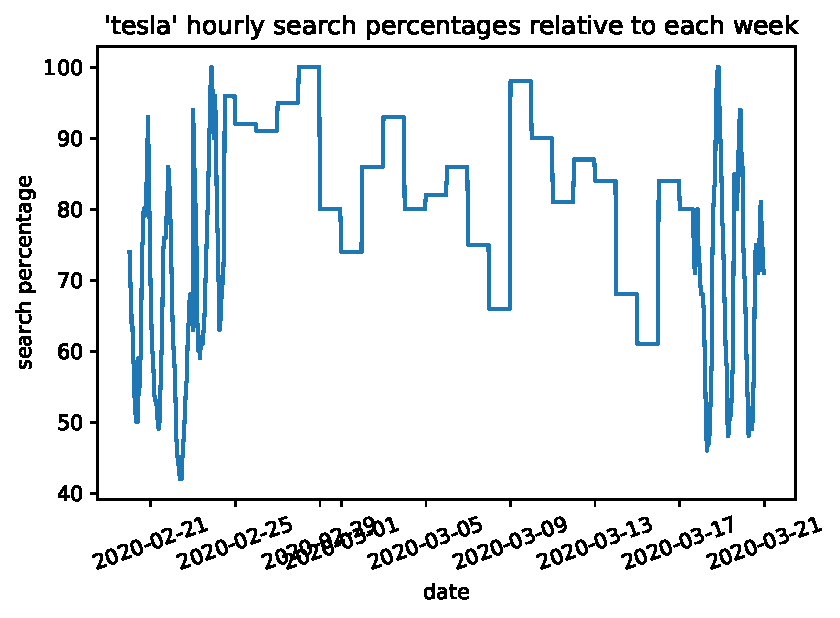
\includegraphics[width=\textwidth]{img/img_GT_tesla_probarea.pdf}
	\caption{Google searches for "tesla" between February 20th and March 20th 2020, where the missing hourly data as truncated with daily data}
	\label{fig:GT_tesla_probarea}
\end{figure}

We observe in this figure also, that there seems to be some daily periodicity in the searches, which is explained by the fact that we only looked at searches done in the United States, so during night time hours it makes sense that there would be less searches.
%Note to self: should I detrend the data ? Or should I look for exceedences over a threshold or some other maxima scheme ??


As the trading data is only between 10am and 5pm EST, we simply dropped data outside of that fork. This was a subjective choice, and it can be discussed whether it would not have been better to aggregate the dropped time and incorporate them in the observations somehow. Our reasoning was that if people searched for the terms before the market opening (say at 11pm the previous day), because they were interested in buying, they were likely to search for the term again right before the market opens, in order to make sure no new information came to light in the mean time to change their mind, and thus their interest would still be captured in the used data. Likewise, if someone was searching with the intent on selling, they too would search again prior to making the transaction, in order to double check.

\begin{figure}[h]
	\centering
	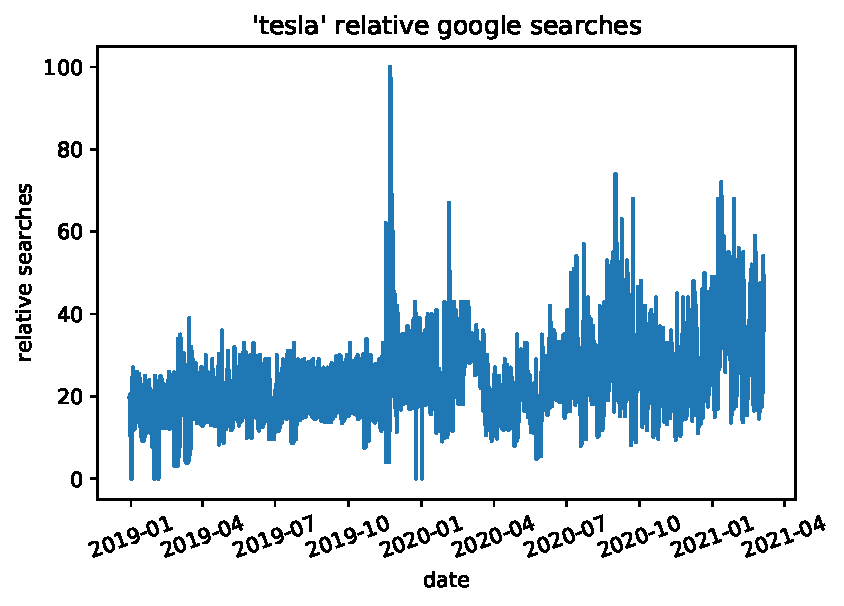
\includegraphics[width=\textwidth]{img/img_GT_tesla.pdf}
	\caption{"tesla" keyword relative google searches}
	\label{fig:GT_tesla}
\end{figure}

The final preprocessed data can be seen in figure \ref{fig:GT_tesla}

\subsection{Twitter data}
The popular social media platform Twitter has an \Gls{API} that lets researchers interact with and explore the Twitter Database. There are several tiers available that give different degrees of access to the database. The free tier did not give significant access to the tweet history, and as such we had to apply for an academic tier.

The API gives access to an impressive amount of data. We will be focusing on tweets by Elon Musk, and twitter metrics of "like count" and "retweet count", though others are available as well. These are the most used metrics when judging a tweets popularity.
Even if they both measure a tweets popularity, if they are not very correlated it could be worth keeping both of them, as a like only shows approval of the tweet, whereas a retweet shows approval, but also spreads the tweet to a larger audience. So it could be used as a metric of how much a tweet has spread.However, upon inspection (Fig  \ref{fig:likeretweets}) the retweet count and the like count seem pretty correlated, so we will focus only on the like count which will be both a measure of the approval of the tweet as well as a measure of how viral it is.

\begin{figure}[h]
	\centering
	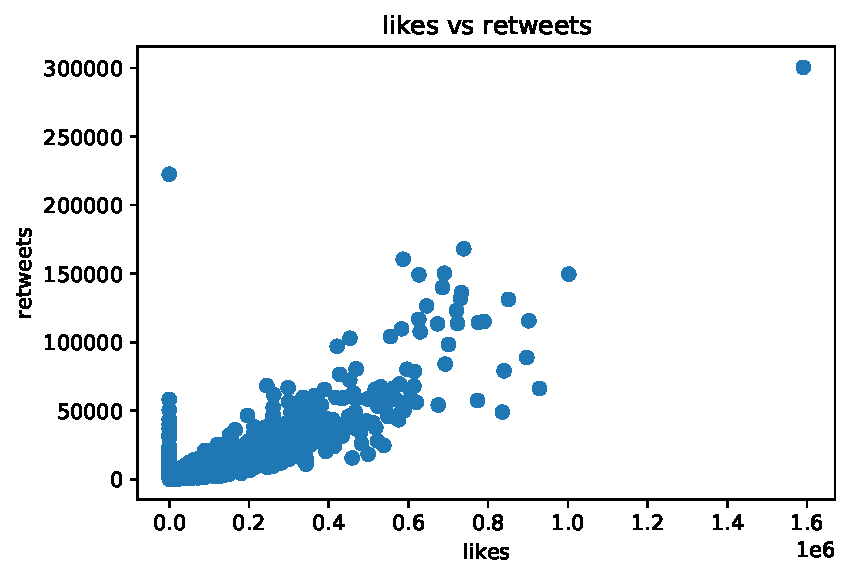
\includegraphics[width=\textwidth]{img/img_likeretweets.pdf}
	\caption{Elon Musk's tweets like count vs retweet count}
	\label{fig:likeretweets}
\end{figure}


Tweets have a precise timestamp and thus we have aggregated them to that for every hour H, the corresponding value is that of the sum of all tweets in the range ]H-1,H]. We then added the out of trading hours values to the first trading hour of each day. Again, it can be discussed whether it would have been better to aggregate this data differently, or drop it all together, like for the \acrlong{gt} data. Our reasoning is that if Elon Musk tweets something out of hours, that gets people in a good or bad frenzy about \acrshort{tsla}, then that frenzy would not die down before the market opened.

Elon Musk tweets a lot about things unrelated to Tesla and it's stock as well, so we will filter tweets with the term "Tesla". This may be too much filtering, as it could be imagined that other keep words could be worth adding to the filter, but it should be decent enough.

\begin{figure}[h]
	\centering
	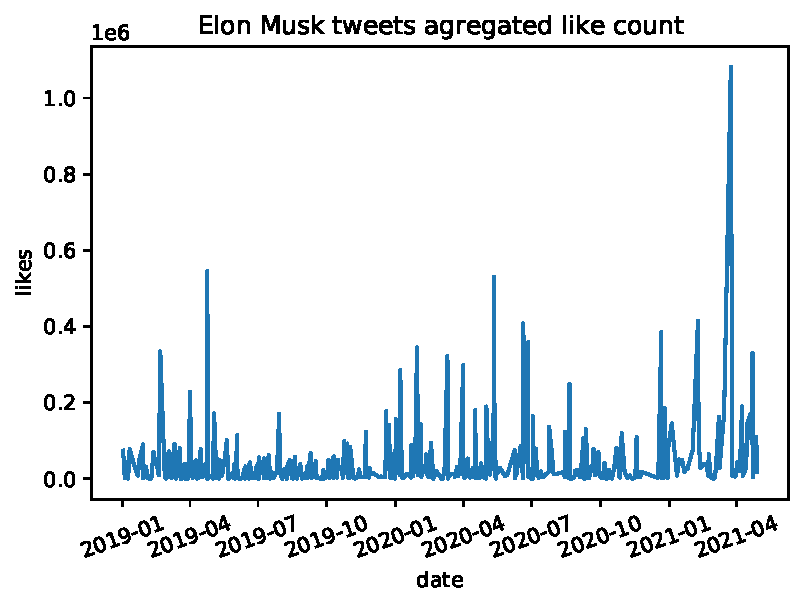
\includegraphics[width=\textwidth]{img/img_agglikes.pdf}
	\caption{Elon Musk's tweets like count, aggregated to fit the trading hours of NASDAQ}
	\label{fig:agglikes}
\end{figure}

The final aggregated like count per period can be seen on figure \ref{fig:agglikes}